%%%%%%%%%%%%%%%%%%%%%%%
% Theoretical Background
%%%%%%%%%%%%%%%%%%%%%%%%

\chapter{Introduction}\label{chap:2}

\section{Overview}
Fluid motions driven by buoyancy and frictional forces belongs to broad class of flows known as thermoconvective shear flows.
These flows exhibit rich behaviour, and are of interest in both engineering and meteorology applications spanning across a broad range of length scales.
At small scales, around $L \sim 1 cm$, the thermoconvection flows are relevant to the cooling of microprocessing chips.
In such systems, the fluid acts medium to dissipate heat, experiences shear forces from the confining walls, and buoyancy from heating.
One of the major innovation in this industry is in squeezing more transistors onto a single chip, resulting to a doubling of transistors on a single chip roughly every two years, according to Moore's law.
% According to Moore's, the amount of transistors on a single chip will double every two years.
However, one of the major limitations on further miniaturisation is the challenge of dissipating the excessive heat generated.
Fluids, such as air, water or refrigerant, are often used to transport heat away from the components, thereby preventing overheating \citep{kennedy_combined_1983, ray_analysis_1992}.
At intermediate length scales, $L \sim 1m$, the interaction between buoyancy and frictional forces is important in the fabrication of uniform thin films in chemical vapour deposition (CVD) \citep{evans_unsteady_1991,jensen_flow_1991}.
The CVD process typically involves a reactive gases carried by inert gases which flows through a channel with a heated substrate.
Upon heating, the reactant gases react chemically at substrate and deposits material, forming thin films, such as silicon layers.
A key challenge in the CVD process is achieving a uniform deposition and maintaining sharp interfaces between layers.
The interactions between shear and buoyancy forces often gives rise to boundary layers and thermoconvective rolls, which can disrupt uniform deposition, affecting fillm quality.
\begin{figure}[ht]
    \centering
    \begin{tikzpicture}[scale=1.3]
        \node at (0,0) {\includegraphics[width=0.2\textwidth]{Background/Figures/Applications/chipcooling.jpg}};
        \node at (0,1.5) {(a) Chip cooling};
        \node at (3.5,0) {\includegraphics[width=0.3\textwidth]{Background/Figures/Applications/CVD.png}};
        \node at (3.5,1) {};
        \node [label={[align=center] (b) Chemical Vapor\\Deposition}] at (3.5,0.7) {};
        \node at (7.8,1.3) {\includegraphics[width=0.3\textwidth]{Background/Figures/Applications/cloudstreets.jpg}};
        \node [label={[align=center] (c) Cloud Streets}] at (7.9, 3.8) {};
        \draw [-, black] (0.1,-1.6) -- (0.1,-1.4);
        \node at (0.1,-1.8) {$10^{-2}$};
        \draw [-, black] (3.5,-1.6) -- (3.5,-1.4);
        \node at (3.5,-1.8) {$10^1$};

        \draw [-, black] (7.5,-1.6) -- (7.5,-1.4);
        \node at (7.5,-1.8) {$10^3$};

        \node [label={[align=center] $L$ $(m)$}] at (9.8,-2.2) {};
        \draw [->, thick, black] (-1,-1.5) -- (10,-1.5);
        % \draw [->, thick, white] (0,-1.8) -- (8.1,-1.8);
    \end{tikzpicture}
    \label{fig:applications}
    \caption{Thermoconvective shear flows driven by shear and bouuyancy forces across length scales, $L \in [10^{-2}m, 10{^3}m]$. Examples include (a) chip cooling, (b) chemical vapour deposition and (c) the formation of cloud streets.}
\end{figure}

At large scales, $L \sim 1km$, the thermoconvective shear flows can be observed in the atmosphere such as the cloud streets over the Norwegian Sea. 
These parallel bands of cumulus clouds can stretch over hundreds of kilometres.
They form when relatively warm sea surfaces heat up the colder air blowing from the North \citep{norwegian_sea}.
As the colder air is heated, it rises upwards whilst carrying water vapour.
As it reaches a certain altitudes, $L \sim 1 - 10km$, the water vapour condenses into visible clouds, while the cooler air falls towards the sea.
This ciruclation is organised into parallel rotating parallel columns of air, forming distinct cloud streets.

The common thread among the examples discussed above is the interaction between shear and bouyancy forces driven fluid motion - the central focus of this thesis.
By restricting our analysis to these two mechanisms, we neglect other physical mechanisms such as phase change, chemical reactions and evaporation, which may be significant in the context of cooling microproccessors, chemical vapour deposition, and atmopsheric boundary layers respectively \citep{vallis_simple_2019}.
To consider this interaction, we consider an idealised setup without geometric complexity, known to as the Rayleigh-B\'{e}nard-Poiseuille (RBP) flow.
This system describes the fluid motion confined between two infinitely extended parallel plates, heated from below and cooled from the top, with an additional pressure gradient driving the flow.
The RBP configuration combines two paradigmatic flow configurations; the classical Rayleigh-B\'{e}nard convection (RBC), driven purely by buoyancy, and plane Poiseuille flow (PPF), driven purely by shear.
While the onset of convection in RBC, and the transition to subscritical shear-driven turbulence in PPF have been both extensively studied, the transitional regime in which both forces interact remains less understood.
Gaining insights into this regime can have implications for various applications across a range of scales mentioned previously. 

\begin{figure}[h]
\centering
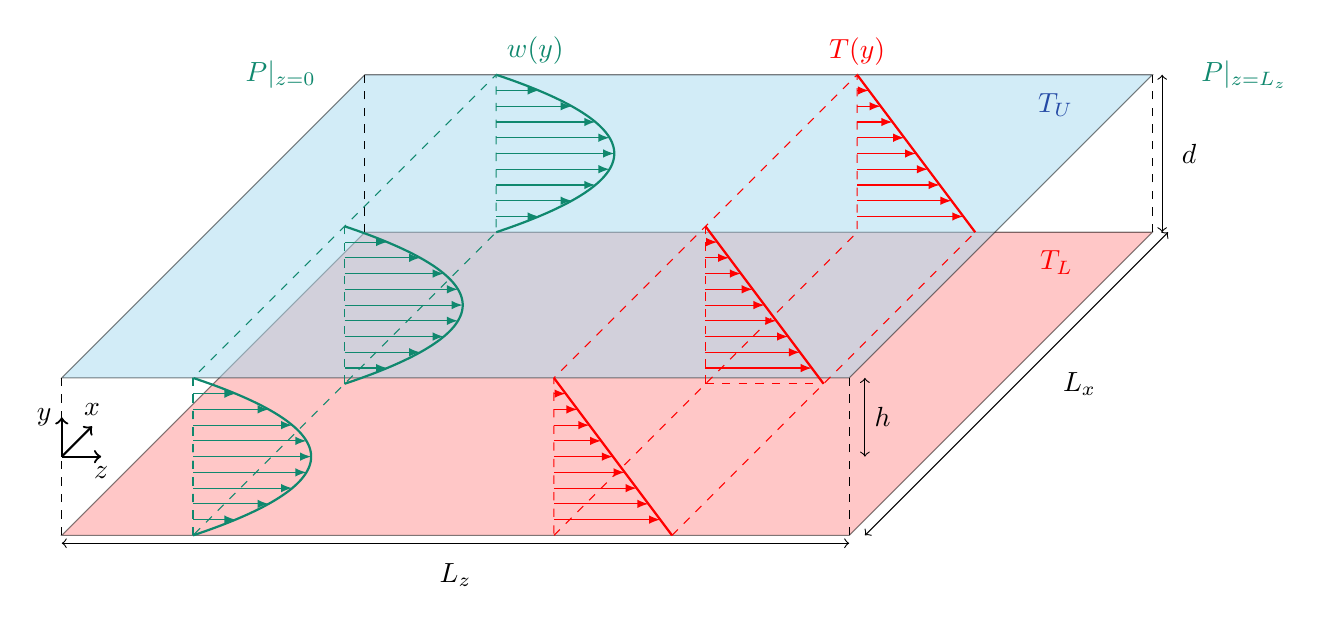
\begin{tikzpicture}
\def\H{1}
\def\W{10}
\def\L{10}

% Draw the bottom plate
\draw [fill=pink!75!red, opacity=0.5] (-\L/2,-\H,0) -- (\L/2,-\H,0) -- (\L/2, -\H, -\W) -- (-\L/2, -\H,-\W) -- cycle;

% Draw the top plate
\draw [fill=SkyBlue!75!white, opacity=0.5] (-\L/2,\H,0) -- (\L/2,\H,0) -- (\L/2, \H, -\W) -- (-\L/2,\H,-\W) -- cycle;

%  % Draw axes
\draw [dashed, thin] (-\L/2, -\H, 0) -- (-\L/2, \H, 0);
\draw [dashed, thin] (\L/2, -\H, 0) -- (\L/2, \H, 0);
\draw [dashed, thin] (\L/2, -\H, -\W) -- (\L/2, \H, -\W);
\draw [dashed, thin] (-\L/2, -\H, -\W) -- (-\L/2, \H, -\W);
%\draw [dashed, thin] (-1,0, 0) --++ (\L,0,0) --++ (0,0,-\W) --++ (-\L,0,0) -- cycle;
%  % \draw [thin, dashed] (-1,0) -- (6,0);

% Add dimensions
% L_x
\draw [<->] (-\L/2,-1.1*\H, 0) -- (\L/2,-1.1*\H,0);
\node[centered] at (0,-1.5*\H,0) {$L_z$};
 
% L_z
\draw [<->] (\L/2*1.025, -\H, -\W) -- (\L/2*1.025, \H,-\W);
\node[right] at (\L/2*1.05,0.0,-\W) {$d$};

% d
\draw [<->] (\L/2*1.04, -\H) -- (\L/2*1.04,-\H,-\W);
\node[centered] at (\L/2*1.2,-\H,-\W/2) {$L_x$};

% h
\draw [<->] (\L/2*1.04, 0, 0) -- (\L/2*1.04, \H, 0);
\node[right] at (\L/2*1.04,\H/2,0) {$h$};

% P
\node[left] at (-\L/2*1.1, \H, -\W) {\textcolor{PineGreen}{$P|_{z=0}$}};
\node[right] at (\L/2*1.1, \H, -\W) {\textcolor{PineGreen}{$P|_{z=L_z}$}};

% T
\node[left] at (\L/2*0.9, \H, -\W*0.9) {\textcolor{cyan!20!blue}{$T_U$}};
\node[left] at (\L/2*0.9, -\H, -\W*0.9) {\textcolor{red}{$T_L$}};

% Draw labels
\draw[->, thick] (-\L/2, 0, 0) -- (-\L/2,\H/2,0) node[left] {$y$};
\draw[->, thick] (-\L/2, 0, 0) -- (-\L/2+\H/2,0,0) node [below] {$z$};
\draw[->, thick] (-\L/2, 0, 0) -- (-\L/2,0,-\H) node[above] {$x$};

% Draw the velocity profile
\draw[PineGreen,thick,domain=-1:1,samples=200,smooth] plot ({(1-\x*\x)*1.5-\L/3}, \x) node[above right] {};
\draw[PineGreen,thick,domain=-1:1,samples=200,smooth] plot ({(1-\x*\x)*1.5-\L/3}, \x, -\W/2) node[above right] {};
\draw[PineGreen,thick,domain=-1:1,samples=200,smooth] plot ({(1-\x*\x)*1.5-\L/3}, \x, -\W) node[above right] {$w(y)$};
\draw[-,PineGreen,dashed] (-\L/3,-\H) -- (-\L/3,\H);
\draw[-,PineGreen,dashed] (-\L/3,-\H, -\W/2) -- (-\L/3,\H, -\W/2);
\draw[-,PineGreen,dashed] (-\L/3,-\H,0) -- (-\L/3,\H,0) -- (-\L/3,\H,-\W) -- (-\L/3,-\H,-\W) -- cycle;

\foreach \y in {-0.8,-0.6,...,0.8} {
    \draw[-latex,PineGreen] (-\L/3,\y, 0) -- ({(1-\y*\y)*1.5-\L/3},\y,0);
    \draw[-latex,PineGreen] (-\L/3,\y, -\W/2) -- ({(1-\y*\y)*1.5-\L/3},\y, -\W/2);
    \draw[-latex,PineGreen] (-\L/3,\y, -\W) -- ({(1-\y*\y)*1.5-\L/3},\y,-\W);
}

% Draw the temperature profile
\draw[red,thick,domain=-\H:\H,samples=200,smooth] plot ({(1/2*(1-\x)*1.5+\L/8)}, \x);
\draw[red,thick,domain=-\H:\H,samples=200,smooth] plot ({(1/2*(1-\x)*1.5+\L/8)}, \x, -\W/2);
\draw[red,thick,domain=-\H:\H,samples=200,smooth] plot ({(1/2*(1-\x)*1.5+\L/8)}, \x, -\W);
\draw[-,red,dashed] (\L/8,-\H,-\W/2) -- (\L/8,\H,-\W/2);
\draw[-,red,dashed] (\L/8,-\H,-\W/2) -- (\L/8 + 1.5,-\H,-\W/2);
\draw[-,red,dashed] (\L/8 +1.5,-\H,0) -- (\L/8 + 1.5,-\H,-\W);
\draw[-,red,dashed] (\L/8,-\H,0) -- (\L/8,-\H,-\W) -- (\L/8,\H, -\W) -- (\L/8,\H,0) -- cycle;
% % 
\foreach \y in {-0.8,-0.6,...,0.8} {
   \draw[-latex,red] (\L/8,\y) -- ({\L/8+(1/2*(1-\y)*1.5},\y);
   \draw[-latex,red] (\L/8,\y, -\W/2) -- ({\L/8+(1/2*(1-\y)*1.5},\y, -\W/2);
   \draw[-latex,red] (\L/8,\y, -\W) -- ({\L/8+(1/2*(1-\y)*1.5},\y, -\W);
}
% Add labels
\node[above,red] at (\L/8,1,-\W) {$T(y)$};
\end{tikzpicture}
\label{fig:rbpconfiguration}
\caption{The Rayleigh-B\'{e}nard Poiseuille (RBP) flow configuration.}
\end{figure}


The RBP configuration is illustrated in figure \ref{fig:rbpconfiguration}, where $z^*, y^*, x^*, L_z, L_x, d, h$ refer to the streamwise, spanwise, wall-normal coordinates, length, span, depth and half-height of the domain respectively.
We note that the asterisks$^*$, refer to variables in dimensional form.
The flow is driven by a pressure gradient along the streamwise $z^*$ direction, $\Delta P^* = P^*|_{z^*=0} - P^*|_{z^*=L_z} < 0$, leading to the formation of a laminar Poiseuille flow, $w^*(y^*)$, for a sufficiently small $\Delta P$. 
In this study, we will only consider fully-developed flow, where the boundary layer from the top and the bottom wall meets at the midplane, $y^*=0$, and entrance effects are neglected.
The RBP configuration is also unstably stratified, such that the temperature difference between the lower, $T_L$, and upper wall, $T_U$, is always positive, $\Delta T = T_L - T_U > 0$, leading to a stable linear conduction profile along the wall-normal direction, $T(y^*)$, if $\Delta T$ is kept sufficiently small.

In the absence of a pressure gradient, the RBP configuration reduces to the classical Rayleigh-B\'{e}nard convection problem, bringing about buoyany-driven convection for a sufficiently large unstable stratification.
In the limiting case without unstable stratification, $\Delta T = 0$, the system reduces to the wall-bounded plane Poiseuille flow (PPF), where the transition towards subscritical shear-driven turbulence may be expected for a sufficiently large pressure gradient.

For instance, do buoyancy forces promote the transition to shear-driven turbulence and how does shear influence the convection? 
To describe the motion of the fluid in RBP configurations, we cosider non-dimensionalised Navier-Stokes equations with Boussinessq approximations,
\begin{subequations}\label{eq:rbp_equations}
\begin{equation}
    \frac{\partial \mathbf{u}}{\partial t} + (\mathbf{u}\cdot\nabla)\mathbf{u} = -\nabla p + \frac{1}{Re}\nabla^2 \mathbf{u} + \frac{Ra}{Re^2Pr} \theta,
\end{equation}
\begin{equation}
    \frac{\partial \theta}{\partial t} + (\mathbf{u} \cdot \nabla)\theta = \frac{1}{RePr}\nabla^2 \theta,
\end{equation}
\begin{equation}
    \nabla \cdot \mathbf{u} = 0.
\end{equation}
\end{subequations}
where $\mathbf{u}(\mathbf{x}), \theta(\mathbf{x}), p(\mathbf{x})$ refers to the nondimensionalised velocity, temperature and presure respectively.
The key control parameters for RBP flows are the Rayleigh number, $Ra$, Reynolds number, $Re$, Prandlt number $Pr$, which are defined as follows,
\begin{equation}
    Ra = \eta g d^3 \Delta T / \nu \kappa, \quad Re = W_c h / \nu, \quad Pr = \kappa / \nu, \quad \Gamma = L/2d,
\end{equation}
where $\eta, g, \Delta T, \nu, \kappa, W_c, h, d, L$ are the thermal expansion coefficient, acceleration due to gravity, temperature difference between the bottom and top wall, kinematic viscosity, thermal diffusivity, laminar centreline velocity, domain's half-depth, full-depth, length or span respectively.

We describe important historical of hydrodynamic stability of planar shear flows and their theorectical frameworks in \S \ref{sec:bkgrd_transitional}.
Theorectical frameworks used in the study of stability of flow such as linear stability, nonlinear dynamical systems and spatiotemporal character of transitional shear flows will be outlined.
This followed the historical developments of Rayleigh-B\'{e}nard convection (RBC), where concepts of the stability of fluid flows will be ultilised in \S \ref{sec:bkgrd_RBC}.
After which, we describe the historical developments of RBP flows \S \ref{sec:bkgrd_RBP}, and the outline of the thesis will be give in \S \ref{sec:thesis_outline}.


% We first discuss the key developments of plane Poiseuille flow (PPF) outlining the key theoretical framework for analysing the stability of fluid flows. This is then followed by Rayleigh-B\'{e}nard convection (RBC) in \S \ref{sec:bkgrd_RBC}.

%%%%%%%%%%%%%%%%%%%%%%%%
% Plane Poiseuille Flows
%%%%%%%%%%%%%%%%%%%%%%%%

\section{Transitional wall-bounded shear flows}\label{sec:bkgrd_transitional}
Wall-bounded shear flows concerns the motion of the fluid flowing in parallel to walls, typically bounded by one or more walls.
The fluid closest to the wall comes to a rest, satisfying the no-slip boundary condition in the presence of a wall.
As a consequence, a velocity gradient in the direction perpendicular from the wall develops, where the fluid layer becomes \emph{sheared} due to the pressence of the wall - referred to wall-bounded sheared flows.
% In Newtonian fluids, shear stresses are directly proportionate to the velocity gradient by the fluids kinetic viscosity, $\nu$, given as,
% \begin{equation}\label{eq:shear}
%    \tau = \nu \frac{\partial u}{\partial y},
% \end{equation}
% where $\tau$, $\nu$, and $\frac{\partial u}{\partial y}$ refers to shear stresses - hence wall-bounded shear flows.
Example of wall-bounded shear flows include the pressure-driven plane Poiseuille flow (or channel flow), Hagen-Poiseuille (or pipe) flows, plane Couette flow and flat plate boundary layers.
These geometrically simple examples enables a convenient framework amenable to the mathematical analysis of fluid motion subjected to shear.
Depending on the degree of shear, the fluid motion can be either laminar, where the fluid layers move in smooth parallel 'laminates', or turbulent, characterised by chaotic eddying motions.
We also note that there is a transitional regime where both states can coexist discuss later.
A central question is predicting the transition from the laminar regime to the turbulence.
% One of the central questions is on the prediction on the transition to turbulence, specifically, when is turbulence expected as shear is increased?
% plane Poiseuille flow (PPF) describes the motion of a fluid confined between two infinitely extended parallel walls, driven by a pressure gradient, also referred to as channel flow.
% It belongs to a general class of wall-bounded shear flows, consisting of plane Couette flow, pipe (Hagen-Poiseuille) flow and flat plate boundary layer flow.

The earliest investigation into this transition dates back to the pipe flow experiments of \cite{reynolds_xxix_1883}.
In his experimental setup, the flow speed through the pipe could be controlled by regulating the inlet pressure, while injecting dye to visualise the flow, as illustrated in figure \ref{fig:reynolds}(a).
At low speeds, the fluid remained laminar, resulting to a single streak of steady dye in figure \ref{fig:reynolds}(b).
As the speed increased, the dye begin to exhibit irregular `sinuous' motions interspersed with laminar regions shown in figure \ref{fig:reynolds}(c).
This is now referred to as the transitional/intermittent regime, alternating between the laminar and turbulent states.
Beyond a critical speed, the dye breaks down entirely into chaotic `eddies', mixing with the surrounding fluid and discolouring the flow with dye downstream in figure \ref{fig:reynolds}(d).
This regime is now identified as turbulence.

Reynolds conjectured that the threshold between the laminar, transitional and turbulent regimes could be characterised by the Reynolds number, $Re = U D/\nu$, where $U$ is the centerline velocity in the pipe, $D$, the pipe diameter and $\nu$, the kinematic viscosity.
He observed that flow through the pipe remained `stable' and laminar for $Re < 1900$, while it became `unstable' and turbulent for $Re > 2000$ \citep{reynolds_iv_1895}.
His remarks led to the concept of the stability of fluid flows.
\begin{figure}[h]
    \centering
    \includegraphics[width=1\textwidth]{Background/Figures/Reynolds.pdf}
    \caption{(a) Osbourne Reynolds pipe experiment with the dye injection apparatus, illustrating the (b) laminar flow, (c) intermittent regime and (d) turbulent flow as the flow speed is increased, taken from \citep{reynolds_xxix_1883}.}
    \label{fig:reynolds}
\end{figure}

%%%%%%%%%%%%%%%%%%%%%%%%%%%
% Linear Stability Analysis
%%%%%%%%%%%%%%%%%%%%%%%%%%%

\subsection{Linear Stability Analysis}
Following Reynolds' experiment, interest towards the mathematical analysis of the stability of fluid flows grew in early $20^{st}$ century.
The mathematical approach typically begins by decomposing the velocity field, $\mathbf{u}(\mathbf{x},t)$, into a laminar (base) state, $U(y)$ (assumed to depend only on the wall-normal direction here), and the velocity perturbations, $\mathbf{u}'(\mathbf{x},t)$, with pressure similarly decomposed as,
\begin{equation}
    \mathbf{u}(\mathbf{x}) = U(y) + \mathbf{u}'(\mathbf{x},t), \quad \text{and} \quad p(\mathbf{x},t) = P(x) + p'(\mathbf{x},t).
\end{equation}
Next, we the substitute the formulations for the decomposed velocity and pressure into the Navier-Stokes equations of equation \eqref{eq:rbp_equations} and drop the nonlinear pertubrations terms $(\mathbf{u'}\cdot \nabla)\mathbf{u'}$,
\begin{subequations}\label{eq:shear_linearised}
\begin{equation}
    \frac{\partial \mathbf{u'}}{\partial t} + (U \cdot\nabla)\mathbf{u'} + (\mathbf{u'}\cdot\nabla)U= -\nabla p' + \frac{1}{Re}\nabla^2 \mathbf{u'},
\end{equation}
\begin{equation}
    \nabla \cdot \mathbf{u}' = 0,
\end{equation}
\end{subequations}
resulting to the linearised Navier-Stokes equations. 
This commonly followed by introducing a wavelike ansatz (mode) defined by streamwise and spanwise wavenumbers, $\alpha, \beta$ and complex frequency, $\omega$.
In general two ways to analysis the linearised Navier-Stokes equations by considering the behaviour of each mode independently in \S \ref{subsec:modal} and their coupled dynamics in \S \ref{subsec:nonmodal}

%%%%%%%%%%%%%%%%%
% MODAL STABILITy
%%%%%%%%%%%%%%%%%

\subsubsection{Modal analysis}\label{subsec:modal}
It is covenient to eliminate the pressure terms by to transform equation \eqref{eq:shear_linearised} using the wall-normal perturbation velocity, $v'$, and wall-normal vorticity, $\eta' = \partial u'/ \partial z - \partial w' / \partial x$, variables.
Using $(v, \eta)$, introduce an ansatz (mode) for them,
\begin{equation}\label{eq:shear_ansatz}
    v'(\mathbf{x},t ) = \tilde{v}(y)e^{i(\alpha x + \beta z - \omega t)}, \quad \text{and} \quad \eta'(\mathbf{x}, t) = \tilde{\eta}(y)e^{i(\alpha x + \beta z - \omega t)}.
\end{equation}
where $\alpha, \beta, \omega$ denotes the streamwise and spanwise wavenumbers, and complex frequency (i.e. $\omega = \omega_r + i\omega_i$), respectively.
Next, we substitute the ansatz into equation \ref{eq:shear_linearised}, leading to the classical Orr-Sommerfeld and Squire equations \citep{orr_stability_1907,sommerfeld_beitrag_1909,squire_stability_1933, schmid_stability_2001},
\begin{equation}\label{eq:OSQ}
    \left[
    -i\omega 
    \begin{pmatrix}
        k^2 - \mathcal{D}^2 & 0 \\
        0 & 1 
    \end{pmatrix}
    + 
    \begin{pmatrix}
        \mathcal{L}_{OS} & 0 \\
        i\beta U' & \mathcal{L}_{SQ} 
    \end{pmatrix}
\right ]
    \begin{pmatrix}
        \tilde{v} \\
        \tilde{\eta}
    \end{pmatrix}
    = \mathbf{0},
\end{equation}
where $\mathcal{L}_{OS}$ and $\mathcal{L}_{SQ}$ refers to the Orr-Sommerfeld and Squire operators given as,
\begin{subequations}
  \begin{equation} 
      \mathcal{L}_{OS} = i\alpha U(k^2-\mathcal{D}^2) + i\alpha U'' + \frac{1}{Re}(k^2 - \mathcal{D}^2)^2,
  \end{equation}
  \begin{equation} 
      \mathcal{L}_{SQ} = i\alpha U + \frac{1}{Re}(k^2 - \mathcal{D}^2).
  \end{equation}
\end{subequations}
$k^2, \mathcal{D}, U', U''$ denotes the sum of squared wavenumbers, $k^2 = \alpha^2 + \beta^2$, differential operator in $y$, first- and second- derivative of the laminar velocity, respectively.
Equation \eqref{eq:OSQ} is simply an eigenvalue problem which could be represented as,
\begin{equation}
    \mathbf{L}\mathbf{\tilde{q}} = i\omega\mathbf{M}\mathbf{\tilde{q}}
\end{equation}
    where,
\begin{equation}
    \mathbf{L} = \begin{pmatrix}
        \mathbf{L}_{OS} & 0 \\
        i\beta U' & \mathcal{L}_{SQ}
    \end{pmatrix},
    \quad \mathbf{M}
    \begin{pmatrix}
        k^2 - \mathcal{D}^2 & 0 \\
        0 & 1 
    \end{pmatrix}, 
    \quad \mathbf{\tilde{q}} = 
    \begin{pmatrix}
        \tilde{v} \\
        \tilde{\eta}
    \end{pmatrix}.
\end{equation}
and $i \omega$ refers to the eigenvalue.
The aim of linear stability analysis is to determine the critical Reynolds number, $Re_c$, which is defined as the lowest value of $Re$ over $\alpha$ and $\beta$, such that $Im[\omega] = 0$.
For $Re > Re_c$, perturbations could grow exponentially, departing from the laminar state.
In other words, we consider the behaviour of each $\alpha-\beta$ mode independently, herein referred to as \emph{modal} analysis.
Squire's theorem implies that for any unstable three-dimensional perturbations, $\beta \neq 0$, there exist an unstable two-dimensional perturbation, $\beta = 0$ with a lower $Re_c$ \citep{squire_stability_1933}.
Therefore, the unstable perturbations of wall-bounded shear flows at $Re_c$ must be two-dimensional.
The theoretical calculations was first perform by \cite{tollmien_uber_1928} and \cite{schlichting_zur_1933} for a flat-plate boundary layer flow, yielding a critical Reynolds number based on streamwise distance $x$ of $Re_{x,c} = Ux_c / \nu = 520$ \citep{schlichting_onset_2017}.
In their honour, the unstable two-dimensional perturbations of the Orr-Sommerfeld operator is referred to as Tollmien-Schlicting (T.S) waves.
For plane Poiseuille flow \citep{orszag_accurate_1971} with a critical wavenumber of $\alpha_c = 1.02$.
However, turbulence in plane Poiseuille flows have been observed at much lower Reynolds number, $Re \sim 1000 - 2000$, contradicting the results from linear stability analysis.
Likewise, the onset of turbulence appear near $Re_{x,c} \approx 5 \times 10^5$ for flat plat boundary layer.
% The aim of linear stability analysis it to search for eigenvalues across $\alpha, \beta, Re$, such that $w_i \geq 0$, denoting an exponential growth of perturbations above a critical Reynolds number defined as $Re_c= \min(\alpha, \beta, Re)|_{\omega = 0}$.
% Interestingly, linear stability analysis for pipe flow predicts a stable laminar flow for all Reynolds numbers \citep{romanov_stability_1973}, contradicting experiments \citep{reynolds_xxix_1883,avila_onset_2011}.
A similar result holds for the plane Couette flow \citep{meseguer_linearized_2003}.
% The critical Reynolds number for the onset of unstable infinitesimal perturbutations in plane Poiseuille flow (PPF) occurs at $Re_{c} = 5772.2$ \citep{orszag_accurate_1971}.
Despite its limitation, linear analysis analysis succeeds in predicting the critical Rayleigh number in Rayleigh-B\'{e}nard convection.
% Despite it failures, it has succeeded in other configurations, such as Rayleigh-B\'{e}nard convection, and Taylor-Couette flow \citep{bodenschatz_recent_2000}, predicting the onset of convection and Taylor rolls are the correct critical parameters.

%%%%%%%%%%%%%%%%%%%%%
% Non-modal stability
%%%%%%%%%%%%%%%%%%%%%

\subsubsection{Non-modal stability}\label{subsec:nonmodal}
One of a major limitation of linear stability analysis considered above is that it treats each eigenmode independently, referred to as \emph{modal} analysis.
However, the interaction between decaying eigenmodes may lead to a short-term amplification of perturbations, before eventually decaying.
This phenonemon is referred to as \emph{transient growth}, and the method of analysis is referred to as \emph{non-modal} analysis, related to the normality of the linear Orr-Sommerfeld operator \citep{schmid_nonmodal_2007}.
\begin{figure}[h]
    \centering
    \includegraphics[width=\textwidth]{Background/Figures/PhasePotrait.pdf}
    \caption{(a) The phase portrait of the toy model with $Re = 15$, (b) Transient growth.}
    \label{fig:toy_model}
\end{figure}
To demonstrate an example of transient growth, we consider a two-dimensional toy model governing the time-evolution of $\mathbf{q}$,
\begin{equation}
    \frac{\mathrm{d}}{\mathrm{d}t} \begin{pmatrix} v \\ \eta \end{pmatrix}  = \begin{pmatrix} -\frac{1}{Re} & -1 \\ 0 & -\frac{2}{Re} \end{pmatrix} \begin{pmatrix} v \\ \eta \end{pmatrix},
\end{equation}
where $Re$ refers to the Reynolds number.
The toy model is has negative eigenvalues, $(\lambda_1, \lambda_2) = (-1/Re, -2/Re)$, and unit eigenvectors $\mathbf{x_1} = (1, 0)$, $\mathbf{x_2} = \frac{1}{\sqrt{Re^2 + 1}}(Re, 1)$.
Judging from the negative eigenvalues, we conclude that $\mathbf{q}(t)$ will decay exponentially.
However, as $Re \rightarrow \infty$, they becoming increasingly non-orthogonal approaching each other such that the angle between $\mathbf{x}_1$ and $\mathbf{x}_2$ tend towards 0.
At $Re = 15$, the eigenvector pairs, $\mathbf{x_1}$ and $\mathbf{x_2}$, are highly non-orthogonal, becoming almost linear dependent shown in figure \ref{fig:toy_model}(a).
For a randomly selected initial condition with an energy-norm of $||\mathbf{q}_0||_2 = 15$, where $|| \cdot ||_2$ refers to the L2-norm, the trajectory in green decays exponentially for $t \in [0, 100]$ in figure \ref{fig:toy_model}(b).
In constrast, for a specifically chosen initial condition in shown as the blue trajectory, $||\mathbf{q}||_2$ is amplified nearly four times before decaying exponentially.
The toy model demonstrates the significance of transient growth for a specifically chosen initial condition.

The goal of non-modal stability analysis is to searching over all initial conditions, $\mathbf{\tilde{q}}_0$, leading to the maximum amplification factor at time $t$, resulting in an optimisation problem,
\begin{equation}\label{eq:transient_growth}
    % G(t) = \max_{\mathbf{\tilde{q}}_0 \neq 0 } \frac{||\mathbf{\tilde{q}}(t)||^2}{||\mathbf{\tilde{q}}_0||^2}, \quad \text{s.t} \quad ||\mathbf{\tilde{q}}_0||^2 = 1,
    G(t) = \max_{\mathbf{\tilde{q}}_0 \neq 0 } \frac{\langle \mathbf{\tilde{q}}(t), \mathbf{\tilde{q}}(t) \rangle }{\langle \mathbf{\tilde{q}}_0, \mathbf{\tilde{q}}_0 \rangle }, \quad \text{s.t} \quad \langle \mathbf{\tilde{q}}_0, \mathbf{\tilde{q}}_0 \rangle = 1,
\end{equation}
where, $\langle \cdot, \cdot \rangle$ refers to the inner-product defined as,
\begin{equation}
    \langle \mathbf{x}, \mathbf{y} \rangle = \int_\Omega \mathbf{x}^H \mathbf{y} \; \mathrm{d}\Omega,
\end{equation}
and $\mathbf{x}^ H$ refers to the complex conjugate transpose of $\mathbf{x}$.
By considering the linearised operator of \eqref{eq:OSQ}, we can define a linear time invariant operator given as,
\begin{equation}\label{eq:linear_evolution}
    \mathbf{\tilde{q}}(t) = \mathcal{A}(t) \mathbf{\tilde{q}}_0,
\end{equation}
which takes the solution from initial conditions, $\mathbf{\tilde{q}}_0$, to $\mathbf{\tilde{q}}(t)$ at time $t$.
Subtituting the expression above into equation \eqref{eq:transient_growth},
\begin{equation}\label{eq:transient_growth_adj}
    G(t) = \max_{\mathbf{\tilde{q}}_0 \neq 0 } \frac{\langle \mathcal{A}(t)\mathbf{\tilde{q}}_0, \mathcal{A}(t)\mathbf{\tilde{q}}_0 \rangle }{\langle \mathbf{\tilde{q}}_0, \mathbf{\tilde{q}}_0 \rangle} = \langle \mathbf{\tilde{q}}_0, \mathcal{A}^\dagger(t) \mathcal{A}(t)\mathbf{\tilde{q}}_0  \rangle = \lambda_{max} (\mathcal{A}^\dagger \mathcal{A})
\end{equation}
where $\mathcal{A}^\dagger(t)$ refers to the adjoint of $\mathcal{A}(t)$. The maximum amplification factor $\max G(t)$ is the largest eigenvalue, $\lambda_{max}$, of $\mathcal{A}^\dagger \mathcal{A}$, and the eigenvalue problem is given as,
\begin{equation}
    \mathcal{A}^\dagger(t)\mathcal{A}(t) \mathbf{\tilde{q}}_0 = \lambda \mathbf{\tilde{q}}_0,
\end{equation}
where $\mathbf{\tilde{q}}_0$ refers to the eigenvector denoting the optimal initial condition.
For a detailed derivation of the optimal initial conditions or forcing, the reader is referred to \citep{butler_three-dimensional_1992,schmid_nonmodal_2007}.
An alternative method of computing transient growth is computing the pseudospectral of linear operators discussed in \citep{trefethen_pseudospectra_1997}, outside the scope of this thesis.

Both two-dimensional, $\beta = 0$, and three-dimensional, $\beta \neq 0$, non-modal stability analysis have been studied.

In the two-dimensional form, the optimal initial conditions are in the form of near wall vorticies tilted upstream, transiently energised referred to as the Orr-mechanism \citep{orr_stability_1907, farrell_optimal_1988,reddy_pseudospectra_1993}.
In the three-dimension form, streamwise vortices, acting as optimal initial conditions lead to the optimal response in the form of streamwise streaks \citep{reddy_energy_1993}.
Contrary to linear stability analysis which confers two-dimensional perturbations as linearly unstable, the key result in this analysis is that three-dimensional initial conditions, $\alpha = 0$, confer the optimal initial conditions leading to large transient growth at subcritical Reynolds numbers.
Figure.. shows this.

The width of the streaks happen to be robustly occur around 100 wall units, the characteristics spacing identified in many experiments [Kline, Panton, Bandybopobi]

The optimal initial conditions involve streamwise vortices which amplify streaks, related to the lift-up effect \citep{ellingsen_stability_1975,brandt_lift-up_2014}.
These modal and nonmodal mechanisms above highlight developments based on linear methods.

% \begin{equation}
%     \langle \mathcal{A}(\tau)\mathbf{x}, \mathbf{y} \rangle = \langle \mathbf{x}, \mathcal{A}^\dagger(\tau) \mathbf{y} \rangle.
% \end{equation}
% Next, we convert the constraint optimisation \eqref{eq:linear_growth_adj} into an unconstraint Lagrangian using Lagrange multipliers,
% \begin{equation}
%     \mathcal{L} = \langle \mathbf{\tilde{q}}_0, \mathcal{A}^\dagger\mathcal{A}\mathbf{\tilde{q}}_0 \rangle  + \lambda (\langle \mathbf{\tilde{q}}_0, \mathbf{\tilde{q}}_0 \rangle - 1)
% \end{equation}
% \begin{equation}
%     \delta L / \delta \mathbf{\tilde{q}}_0 = 2 \mathcal{A}^\dagger\mathcal{A}\mathbf{\tilde{q}}_0 - 2\lambda \mathbf{\tilde{q}}_0 = 0,
% \end{equation}
% where $\lambda$ refers to the Lagrange multiply.
% By invoking the optimal conditions, $\delta L/ \delta \mathbf{\tilde{q}}_0 = 0$, we get,
% \begin{equation}
%     \mathcal{A}^\dagger\mathcal{A}\mathbf{\tilde{q}}_0 = \lambda \mathbf{\tilde{q}},
% \end{equation}

% The maximum amplification factor $G(\tau)$ is simply the maximum eigenvalue of $\mathcal{A}^\dagger(\tau) \mathcal{A}(\tau)$, expressed as,
% Next, we describe the transient approach for Orr-Sommerfeld problem, by first casting it in its time-evolution form,
% \begin{equation}
%     \frac{\partial}{\partial t} \mathbf{\tilde{q}} = 
%     \begin{pmatrix}
%         (D^2 - k^2)^{-1}\mathcal{L}_{OS} & 0 \\
%         -i\beta U' & -\mathcal{L}_{SQ}
%     \end{pmatrix}
%     \mathbf{\tilde{q}},
% \end{equation}
% Next, we consider the evolution equations of the Orr-Sommerfeld operator as,
% where the solution at time $\tau$ is given as,
% \begin{equation}
%     \mathbf{\tilde{q}}(\tau) = \exp(\mathcal{A}\tau) \mathbf{\tilde{q}}_0
% \end{equation}
% where $\mathbf{A} \mathbf{V}= \mathbf{V}\mathbf{D}$ is diagonalisable where $\mathbf{V}, \mathbf{D}$ refer to the eigenvectors and values respectively.
% 
% \begin{equation}
%     G(t) = \max_{\mathbf{\tilde{q}_0} \neq 0} \frac{||\mathbf{\tilde{q}}(t)||^2}{||\mathbf{\tilde{q}}_0||^2}, \quad \text{s.t} \quad ||\mathbf{\tilde{q}_0}||^2 = 1.
% \end{equation}
% The energy-norm is defined with a continuous inner-product,
% \begin{equation}
%     ||\mathbf{x}
% \end{equation}
% \begin{equation}
%     ||\mathbf{\tilde{q}}(t)||^2 = \langle \mathbf{A}(t) \mathbf{\tilde{q}_0}, \mathbf{A}(t) \mathbf{\tilde{q}_0} \rangle = \int_\Omega (\mathbf{A}\mathbf{\tilde{q}})^* \mathbf{A}\mathbf{\tilde{q}} \; \mathrm{d} \Omega,
% \end{equation}
% where $\cdot^{*}$ refer to the complex conjugate.
% Next, we introduce the adjoint operator where,
% \begin{equation}
%     \langle \mathbf{x}^\dagger, A x \rangle = \langle A^\dagger \mathbf{x}, \mathbf{x} \rangle
% \end{equation}
% \begin{equation}
%     G(t) = \max_{\mathbf{\tilde{q}_0} \neq 0} \frac{||\mathbf{\tilde{q}}(t)||^2}{||\mathbf{\tilde{q}}_0||^2} = \max_{\mathbf{\tilde{q}_0} \neq 0} \frac{\mathbf{a_0}^T\exp(\mathbf{D}t)\mathbf{V}^T\mathbf{V}\exp(\mathbf{D}t)\mathbf{a}_0}{\mathbf{a}_0^T \mathbf{V}^T \mathbf{V} \mathbf{a}_0}
% \end{equation}
% \begin{equation}
%     G(t) = \max_{\mathbf{\tilde{q}_0} \neq 0} \frac{||\mathbf{\tilde{q}}(t)||^2}{||\mathbf{\tilde{q}}_0||^2} = \max_{\mathbf{\tilde{q}_0}} \frac{\mathbf{\tilde{q}_0}^T \mathbf{A}^T \mathbf{A} \mathbf{\tilde{q_0}}}{\mathbf{q}_0^T\mathbf{q}_0}
% \end{equation}
%%%%%%%%%%%%%%%%%%%%%%%%%%%%%
% NONLINEAR DYNAMICAL SYSTEMS
%%%%%%%%%%%%%%%%%%%%%%%%%%%%%

\subsection{Nonlinear dynamical systems}

\begin{figure}[h]
    \centering
    \includegraphics[width=0.8\textwidth]{Background/Figures/StateSpaceGraham.png}
    \caption{The state space organising of the upper and lower branch. Turbulence is interpreted as solution trajectories wander around the upper branch, orbiting around a network unstable invariant states. The lower branch acts as a boundary between the turbulent attractor and laminar attractor, an attracttor on the edge referred to as the edge state. Taken from \citep{graham_exact_2021}.}
    \label{fig:StateSpaceGraham}
\end{figure}

In the previous section, we have examined the transition process based linear mechanisms.
Unfortunately, for canonical shear flow configurations, the transition process is subscritical where linear stability theory fails to predict the onset of turbulence.
Furthermore, the transition to turbulence is ultimately governed fully nonlinear nature of the Navier-Stokes equations.
Hence, we turn to a nonlinear dynamical systems point of view of this transition process, inspired from Hopf's vision of transition, where turbulence emerge as a chaotic trajectory after succeeding Hopf bifurcations.. [CHECK THIS DESCRIPTION...]
However, this bifurcation cannot happen in the subcritical 
In this view, turbulence is interpreted as a solution trajectory evolving through a phase space composed of a network such non-trivial nonlinear solutions, commonly referred to as exact coherent states (ECS) or invariant solutions \citep{graham_exact_2021}.

In the context of parallel shear flows, Nagata was the first to discover a pair of unstable equilibirum solutions in plane Couette flow by smoothly following (homotopy) from a Taylor-Couette configuration \citep{nagata_three-dimensional_1990}.
This pair consist of an unstable upper branch and lower branch emerging as a saddle-node bifurcation near $Re \approx 500$, and is disconnected from the stable laminar solution.
The lower branch refers to its proximity towards the stable laminar state in phase space.
A travelling-wave solution in plane Couette flow also later found by the same author \citep{nagata_three-dimensional_1997}.
A family of equilibrium and travelling waves solutions was found for plane Couette and plane Poiseuille flows under various boundary conditions (i.e. stress-free, slip and no-slip) where identified by \citep{waleffe_exact_2001,waleffe_homotopy_2003}.

While these unstable solutions demonstrate good agreements with results from DNS such as the spanwise length scales, and mean and fluctuations, they do not capture the dynamical processes.
Periodic orbits defined by time-dependent solutions that have been identified in plane Couette flow \citep{kawahara_periodic_2001}, describing a single regeneration cycle similar to the self-sustaining process.
The chaotic trajectories of turbulence have been found to be embedded within invariant solutions and their connections between them known as heteroclinic orbits, offering a robust view of the building-blocks of of turbulence \citep{gibson_visualizing_2008, gibson_equilibrium_2009, viswanath_recurrent_2007, halcrow_heteroclinic_2009, graham_exact_2021}

In the context of this transitional flows, the lower branch solution can be though of separating the turbulent attractor from the laminar state.
Its an attractor that resides on the edge of turbulence, defined as an edge state.
The graphical representation of this edge is shown in figure \ref{fig:StateSpaceGraham}.

% Coherent structures and turbulent motions
These invariant solutions commonly take the form of as equilibria, travelling waves, periodic and relative periodic orbits.
It is well established that coherent motions defined by flow patterns that persist in space and time play an important role in the transport of momentum and heat.
In parallel shear flows, these coherent structures typically appear as near-walls streaks and quasi-streamwise rollers.
A persistent, quasi-periodic cycle between the regeneration of streaks and rolls, referred to as the \emph{self-sustaining process}, appears to be a fundamental mechanism in sustaining wall-bounded turbulence \emph{self-sustaining process} \citep{hamilton_regeneration_1995}.
This mechanism is described by the generation of streaks due to quasi-streamwise rollers by redistributing the mean.
These streaks become linearly unstable and breakdown, and through a nonlinear process regenerates the quasi-streamwise rollers, closing the cycle.

% Utilising tools from nonlinear dynamics systems, turbulence could be viewed as chaotic trajectories around unstable nonlinear solutions known as invariant solutions or exact coherent structures \citep{Waleffe_2001,Waleffe_2003,toh2003periodic,Kreilos_2012,nagata2013mirror,Wall_Nagata_2016,Zammert_Eckhardt_2014,graham21}.

%%%%%%%%%%%%%%%%%%%%%%%%%%%%%%%%%%%
% Spatiotemporal transitional flows
%%%%%%%%%%%%%%%%%%%%%%%%%%%%%%%%%%%

\subsection{Spatiotemporal transitonal flows}
\begin{figure}[h]
    \centering
    \includegraphics[width=\textwidth]{Background/Figures/Re1400.pdf}
    \caption{A snapshot of turbulent-laminar bands at $Re = 1400$ in a large domain $L/d = 8\pi$, depecting its spatiotemporal intermittent nature. Isovolume renderings is based on the spanwise, $u'$, and wall-normal, $v'$, perturbation kinetic energy, $E(u',v') = 1/2(u'^2 + v'^2)$, where the perturbation velocities are defined about the laminar state $\mathbf{u}'(\mathbf{x},t) = \mathbf{u}(\mathbf{x},t) - U_{lam}(y)$.}
    \label{fig:turbulent-laminar}
\end{figure}

This section describes the inherent spatiotemporal intermittent description of turbulence in transitional wall-bounded shear flows commonly reported in large extended domains where the span is about fifty times the half-height of a plane Poiseuille channel, $L/h \gtrsim 50$.
In thie regime, turbulence is characterised by the coexistence of turbulent and laminar structures.
Examples of such are found in canonical shear flow systems such as plane Couette flows \citep{prigent_long-wavelength_2003,barkley_computational_2005,barkley_mean_2007,tuckerman_patterns_2011,duguet_formation_2010,reetz_exact_2019}, Taylor-Couette flows \citep{prigent_barber_2002,prigent_long-wavelength_2003}, pipe flows \citep{avila_transient_2010,avila_onset_2011,song_speed_2017,avila_transition_2023} and plane Poiseuille flows \citep{tsukahara_dns_2014, tsukahara_dns_2014-1, tuckerman_turbulent-laminar_2014, tsukahara_experimental_2014, gome_statistical_2020, paranjape_onset_2019, paranjape_oblique_2020, paranjape_direct_2023}.

We will focus on the plane Poiseuille flow configuration, where the spatiotemporal intermittent patterns are referred to as oblique turbulent-laminar bands illustrated in figure \ref{fig:turbulent-laminar} at $Re = 1400$ for $L/h = 16\pi$.
The the bright and dark regions highlights coexisting spatially localised turbulent and laminar regions.
These turbulent-laminar bands occur over a range of Reynolds numbers, and its precise range is likely dependent on the domain's aspect ratio \citep{tsukahara_experimental_2014,tuckerman_turbulent-laminar_2014,paranjape_direct_2023}.
Near the upper $Re$ threshold of this regime, the domain is fully engulfed by developed turbulent regions, referred to uniform, featureless turbulence appearing at $Re = 1800$ in figure \ref{fig:turbulent-laminar}(a).
As $Re$ decreases towards $Re = 1050$, turbulent-laminar bands persist in figures \ref{fig:turb_lam_bands}(b-f).
In this region, turbulent-laminar bands angles have been observed to be inclined between $20^\circ \sim 30^\circ$, with streamwise wavelengths of $\sim 60h$, and spanwise wavelengths of $\sim 20h-30h$ \citep{tsukahara_experimental_2014}.
To study the preference of angles, zzz performed linear stability analysis of bands and showed that preferred angle at .. degrees.
Below certain $Re$ threshold, the spatially turbulent regions spontaneously decay where the flow relaminarises asymptotically \citep{tuckerman_turbulent-laminar_2014}.
This decay is shown in $Re = 1000$ near $t = 1600$ in figure \ref{fig:turb_lam_bands}(g). 
\begin{figure}[h]
    \centering
    \includegraphics[width=\textwidth]{Background/Figures/Ra0-BotSpaceTime.pdf}
    \caption{Turbulent-laminar bands for $t \in [0, 3000]$ in large domains $(L_x, L_z) = (16\pi, 16\pi)$ at (a) $Re = 1800$, (b) $Re = 1600$, (c) $Re = 1400$,  (d)  $Re =1200$, (e) $Re = 1100$, (f) $Re = 1050$,  (g) $Re = 1000$.}
    \label{fig:turb_lam_bands}
\end{figure}

Inspired from previous studies of turbulent-laminar bands in plane Couette flows \citep{barkley_computational_2005, reetz_exact_2019}, narrow domains, titled orthogonally to the band angles where considered to investigate their dynamics \citep{tuckerman_turbulent-laminar_2014, paranjape_oblique_2020, paranjape_direct_2023}.
In narrow-tilted domains inclined at $24^\circ$, the turbulent-bands convect at about $\sim1\%$ of the bulk velocity, propagating either upstream or downstream, above or below an critical $Re \sim 1000$, independent of domain sizes for $L_z \geq 100h$ \citep{tuckerman_turbulent-laminar_2014,gome_statistical_2020}.
\begin{figure}[h]
    \centering
    \includegraphics[width=0.7\textwidth]{Background/Figures/gome_prob.pdf}
    \caption{The mean decay times (red), $\tau^d$, and mean splitting times (black), $\tau^s$, as a function of Reynolds number, leading to a crossover point at $Re \approx 965$, adapted from \citep{gome_statistical_2020}.}
    \label{fig:decay_split_probability}
\end{figure}
The characteristic spanwise wavelengths of turbulent-laminar bands are depdendent on $Re$, appearing at $\lambda_z \sim 20h$ for $Re \geq 1400$ and $\lambda_z \sim 40h$ for $Re \leq 1100$.
Indeed, between $1300 < Re < 1400$ the bands appear to alternative between two different band-widths \citep{tuckerman_turbulent-laminar_2014}, merging and splitting continuously. 
This points towards a band splitting event in between $Re = 1100$ and $Re = 1400$, reminiscent of a puff splitting in pipe flows \citep{avila_onset_2011}.

On the other hand, turbulent bands appear to decay at $Re = 830$ \citep{gome_statistical_2020}, and at $re = 1100$ but surviving for $re = 1000$ \citep{tuckerman_turbulent-laminar_2014}, suggesting that turbulent bands decay spontaneously.
\citep{gome_statistical_2020} computed the probabilities distributions of turbulent band decay, $P(\Delta t^d)$, where $\Delta t^d$ refers to the time it takes for decay.
On of the key insight is that the probability distributions of turbulent band decay mimicks a memoryless Poisson distribution,
\begin{equation}
    P(\Delta t^d) = \exp(-\Delta t^d/\tau^d(Re)),
\end{equation}
where $\tau^d(Re)$ refers to the mean lifetime for decay as a function of $Re$.
Similarly, the probability distribution for band splitting also follows a Poisson distribution, $P(\Delta t^s) = \exp(-\Delta t^s / \tau^s(Re))$, where $\tau^s(Re)$ refers to the mean lifetime of a splitting event dependent on $Re$.
The mean survival lifetime of a band decaying, $\tau^d$, and splitting, $\tau^s$, depends superexponentially on $Re$, i.e. $\tau^{d,s} = \exp(\exp(Re))$.
This superexponential dependence is presented in figure \ref{fig:decay_split_probability}, with a crossover point at $Re_{cross} \approx 965$.
This crossover point refers to equal mean survival lifetime of a band de
suggesting a critical $Re$ for the onset of turbulent bands.
% By extrapolating the estimated mean lifetimes of a splitting and decay event, the crossing point (i.e equal chance of identifying a splitting and decay event after a time-scale of $t = 3 \times 10^6$) occurs at $Re_{cross} \approx 965$, in other words, $Re_{cross}$ acts as a critical Reynolds number.
While there has substantial progress made towards understanding the behaviour of periodic turbulent-laminar bands in narrow-tilted domains, recently studies of isolated turbulent bands (ITBs) indicate differed behaviour.
Notably, ITBs persist at $Re \approx 700$ for $t = 10000$ (far beyond figure \ref{fig:decay_split_probability}, characterised by streak generating head, and a diffusive upstream tail. \citep{xiong_turbulent_2015, tao_extended_2018, shimizu_bifurcations_2019, xiao_growth_2020}.
% It is worth noting that isolated bands are not memoryless, depending on their pass history [citation]
% Above a certain Reynolds number, the probability of band splitting again depends on a super-exponentianal.
% Show graph.
% In the context of plane Poiseuille flowsd, it is well known that at $Re \sim 1000 - 2000$, turbulence behaves intermittently, existing as oblique bands of turbulent and laminar regions. 
% Over the past decade, research efforts have been dedicated to the study of turbulent-laminar bands.

% At $Re \sim 1000 - 2000$, turbulent bands can either decay spontaneously, stabilising into a laminar state, or split, forming more bands whereby turbulent-laminar bands are sustained.
% The probability of decay and splitting lifetimes strongly depends on the domain size and $Re$.
% At $L_z = 100h$, the critical Reynolds number of $Re_{cr} \approx 965$ have been determined statistically, whereby decay and splitting lifetimes intersect more than $10^6$ advective time units. 
% It is worth to note that for $Re < Re_{cr}$, the probably of decay is higher than splitting events, vice versa. 


%%%%%%%%%%%%%%%%%%%%%%%%%%%%
% Rayleigh Benard Convection
%%%%%%%%%%%%%%%%%%%%%%%%%%%%

\section{Rayleigh-B\'{e}nard convection}\label{sec:bkgrd_RBC}

\begin{figure}[h]
    \centering
    \includegraphics[width=\textwidth]{Background/Figures/BenardCells.png}
    \caption{(a) Surface tension driven convection leading to the onset of hexagonal B\'{e}nard cells in a thin layer of silicone oil, heated from below and cooled by ambient air. A diamond defect appears, likely caused by plate imperfections. (b) Buoyancy driven convection in rigid plates, resulting to concentric convection rolls at $2.9$ times the critical Rayleigh number. Both experiments were performed by \cite{koschmieder_heat_1974}, and the convection patterns were illuminated by aluminum powder, where the dark and bright regions refer to vertical and horizontal motions resepctively. These higher resolution images were taken from \citep{van1982album}.}
    \label{fig:benard_cells}
\end{figure}

Rayleigh-B\'{e}nard convection (RBC) is a paradigmatic fluid configuration describing the motion of the fluid confined between two infinite-parallel plates heated from below and cooled from the top.
% The basic physical mechanism underpinning RBC is variation of buoyancy due to heat, offering a simple description of natural convection.
As the bottom plate is heated, the bottom layer fluid becomes more buoyant and tends to rise, while the colder top fluid layer is becomes relatively less buoyant and tends to sink, leading to an overturning of layers.
Viscous forces between neighbouring fluid parcels act to resist the motion. 
As buoyancy overcomes these viscous forces, the fluid layers overturn, resulting in the initiation of buoyancy-driven convection, the physical mechanism underpinning RBC.

One of the earliest experimental studies dedicated to buoyancy-driven convection was conducted by Henri B\'{e}nard \citep{benard_tourbillons_1901}, who observed the formation of hexagonal convection cells above a certain temperature threshold $\Delta T$.
These hexagonal patterns are referred to as B\'{e}nard cells are illustrated in figure \ref{fig:benard_cells}(a) (adapted from \citep{koschmieder_heat_1974}).
Subsequently, \cite{rayleigh_lix_1916} carried out one of first linear stability analyses of buoyancy-driven convection, predicting the onset of convection at a critical Rayleigh number of $Ra_c = 657.5$.
However, Rayleigh's analysis assumed an idealised free-free boundary conditions, which differed from the rigid-free setup of B\'{e}nard's experiment.
The linear stability analysis for rigid-free configuration was later performed by \cite{jeffreys_cases_1928} yielding a higher critical Rayleigh number of $Ra_c = 1058$.
In the rigid-rigid configuration, the critical Rayleigh number increases further to $Ra_c = 1708$ \citep{pellew_maintained_1940}.
The Rayleigh number in B\'{e}nard's original experiment was found to be 300 to 1500 smaller than $Ra_c$ for the free-free and rigid-free cases \citep{wesfreid_henri_2017}.
% However, it is worth highlighting a key difference in B\'{e}nard's experiment and Rayleigh's analysis.
This contradiction, not recognised by B\'{e}nard at the time, lies in the significant role of surface tension in thin fluid layers exposed to air, now known as B\'{e}nard-Maragoni (BM) convection \citep{block_surface_1956, cloot_nonlinear_1984, manneville_thirty_2006, wesfreid_henri_2017}.
In BM convection, fluid motion is primarily driven by surface tension gradients due to variations of temperature, forming hexagonal cells, as in figure \ref{fig:benard_cells}(a).
The preference for hexagonal cells in BM convection was later confirmed based on weakly nonlinear stability analysis \citep{cloot_nonlinear_1984}.
% as in B\'{e}nard experiments, a thin layer of fluid exposed to the air is chiefly driven by the variation of surface tension due to temperature difference, leading to the growth of hexagonal cells, in figure \ref{fig:benard_cells}(a).
As the fluid layer becomes thicker, surface-tension effects diminish and buoyancy-driven convection becomes dominant.
Similarly, placing a rigid lid on top of a thin fluid layer suppresses surface-tension effects, also resulting in buoyancy-driven convection.
% Surface-tension effects diminish as the fluid depth increases, or removed in the presence of a top rigid lid, where buoyancy becomes the dominant mechanism.
The preferred convection patterns based on weakly nonlinear stability analysis are the two-dimensional parallel rolls, now referred to as ideal straight rolls (ISRs) \citep{schluter_stability_1965, bodenschatz_recent_2000}.
% This also have the same effect as placing a lid on top of thin layer of fluid where surface-tension effects are removed, leading to ISRs.
% This key discrepancy was later identified as B\'{e}nard's experiments considered thin layers of fluid heated and cooled by the ambient air \citep{block_surface_1956}, where surface tension (Maragoni) effects were significant.
In circular ontainers, the ISRs conform to the geometry of the boundaries, forming concentric convection rolls illustrated in figure \ref{fig:benard_cells}(b).
Interestingly, hexgaonal cells have been observed in buoyancy-driven flows of non-Boussinesq fluids \citep{hoard_experiments_1970,bodenschatz_recent_2000}.
In this thesis, I will consider RBC with rigid-rigid boundary conditions with for which the critical Rayleigh number is $Ra_c = 1708$.
Notably, the corresponding critical wavelength is $q_c = 3.12 / d$ (or $\lambda_c \approx  2d$), suggesting that distance separating the plates, $d$, dictates the length of a single roll, $l_{roll} = \lambda_c / 2 \approx d$.
% 1. Bousinessq fluids (silicon oil) leads to 2D rolls or Hexagonal rolls for rigid-rigid and open-rigid B.Cs - highlighting the importance of the top B.C
%     a. Are they buoyancy driven or surface-tension driven?
% 
% 2. Non-bouseinessq (Aroclor) lead to rigid-rigid boundary conditions lead to rolls for thick layers, and hexes in thin layers. In open-rigid boundary conditions, 2D concentric rolls develop in thick layers while hexagonal cells form in thin layers.


% While the $Ra_c$ for free-free and rigid-free have been reported \citep{rayleigh_lix_1916,jeffreys_cases_1928}.
% It is also worth noting that \cite{rayleigh_lix_1916} considered a stress-free boundary conditions in his analysis, which has been extended to rigid boundary conditions, the critical Rayleigh number increased to well known $Ra_c = 1707.8$ \citep{pellew_maintained_1940}, and is independent or $Pr$ \citep{bodenschatz_recent_2000}.

% ension decreases  generated a tangential forces towards regions of higher surface tension at the surface, where cold fluid resides, ampliying convection, now known as B\'{e}nard-Maragoni convection \citep{manneville_thirty_2006}. 
%, with a critical wavenumber of $q_c = \frac{\pi}{\sqrt{2}d}$.
% and predicted the critical Rayleigh number of $Ra_c = \frac{27}{4}\pi^4 = 657.5$, and a critical wavelength of $q_c = \frac{\pi}{\sqrt{2}d}$.
% where $Ra, \alpha, g, d \Delta T, \kappa, \nu$ refers to the Rayleigh number, volumetric thermal expansion of the fluid, gravitational constant, width and temperature difference between plates, thermal diffusivity and kinematic viscosity. 
% When $Ra$ exceeds a certain critical Rayleigh number $Ra_c$, the fluid configuration becomes unstable and convection motion ensures.
% The pioneering work from Rayleigh, and B\'{e}nard's experiment formed the early foundations of buoyancy-driven convection, now known as Rayleigh-B\'{e}nard convection.
% In the absence of surface tension effects, the critical Rayleigh number, $Ra_c$ depends on the boundary condition, commonly analysed using stress-free or rigid-rigid (no-slip) boundary conditions.
% In Rayleigh's work, he considered a stress-free condition at the wall, ${\partial u}/{\partial n} = 0$, where analytical solutions are admittable.

\begin{figure}[h]
    \centering
    \includegraphics[width=0.8\textwidth]{Background/Figures/BusseBalloonFull.png}
    \caption{The Busse ballon describes the stability boundaries of ISRs in a $\varepsilon-q$ space. For larger wavenumbers, the instability mechanisms is described by the skewed-varicose (SV) instability. For smaller wavenumbers, the instability mechanism is described by the Eckhaus instability. For large $\varepsilon$, the instability is described by the onset of oscillatory instability. Busse balloon digitised from \citep{plapp_spiral_1997} for $Pr \approx 1$.}
    \label{fig:busseballon}
\end{figure}

As mentioned earlier, stationary ISRs near $q_c$ emerge just above $Ra_c$, based on weakly nonlinear stabity analysis. \citep{eckhaus_studies_1965, schluter_stability_1965}.
However, this prediction contradicted by the emergence of time-dependent oscillatory ISRs in experiments \citep{rossby_study_1969,willis_oscillatory_1970} at $Ra = 9200$ (or roughly five times $Ra_c$), where weakly nonlinear stability becomes inapplicable far from threshold.
To address this, a direct secondary stability analysis was employed to study the stability of ISRs further from $Ra_c$, based on Galerkin analysis \citep{busse_oscillatory_1972}
% \cite{busse_oscillatory_1972} performed secondary linear stability analysis of ISRs based on Galerkin truncation of orthogonal functions.
The results from the analysis is described by the Busse balloon, which illustrates the stability boundaries of ISRs as a function of $Ra$ and $Pr$ and roll wavenumber, $\alpha$, shown figure \ref{fig:busseballon} \citep{busse_non-linear_1978}.
The boundaries of the Busse balloon are described by a range of secondary instabilities, each arising from different physical mechanisms \citep{busse_non-linear_1978}.
At large Prandtl numbers, $Pr = O(10^2)$, the zig-zag (ZZ) and cross-roll (CR) instabilities delimits the balloon for small and large roll wavenumbers.
The zig-zag instabilities cause zig-zag undulations while the CR instabilities generates rolls orthogonal to the underlying ISR structure, effectively increasing or decreasing the roll wavenumber respectively \citep{busse_instabilities_1971}.
Examples of these instabilities at $Pr = 100$ are illustrated in figure \ref{fig:busseballoon_secinstab}(a,b).

\begin{figure}
    \centering
    \includegraphics[width=0.5\textwidth]{Background/Figures/BusseBalloon/SecondaryInstabilities.pdf}
    \caption{ISRs experiencing (a) cross-roll instability at $Ra = 3000, Pr = 100$ and (b) zig-zag instability at $Ra = 3600, Pr = 100$ \citep{busse_instabilities_1971}. (c) Skew-varicosed instability at $Ra = 5568, Pr = 1$ \citep{plapp_spiral_1997}, and (d) oscillatory instability at $Ra = 10384, Pr = 1$ \citep{cakmur_bistability_1997}.}
    \label{fig:busseballoon_secinstab}
\end{figure}

At moderate Prandtl numbers, $Pr = O(1)$, the Busee balloon is bounded by the skewed varicosed (SV) for high roll wavenumbers and the oscillatory (OS) instability at large $Ra$.
% The cross-roll instability generates an additional roll orthogonal to the existing roll, while the zig-zag instabilities leads to the emergence of zig-zag ISRs.
The skewed-varicosed (SV) instability leads to roll-pinching where pinched rolls merged into a single roll, reducing roll wavenumber while the oscillatory instability leads to the onset of an oscillatory ISRs. 
Examples of the respective instabilities at $Pr = 1$ are shown in figure \ref{fig:busseballoon_secinstab}(c,d).
At higher wavenumbers, the skewed varicose (SV) instability becomes relevant at intermediate Prandlt numbers, characterised by roll pinching and merging that effectively reduces the roll wavenumber.
% For larger Rayleigh numbers and $Pr \lesssim 1$, the oscillatory instability (OS) arises, forming oscillatory ISRs \citep{willis_oscillatory_1970}.
% In contrast, for higher $Pr$, the knot instability appears, modifying the cross-roll pattern into a spoke-like structure.
Finally, the Eckhaus instability (not shown), related to the symmetry of the system, appears close to the $Ra_c$, leading a disturbance parallel to the underlying rolls which either creates or destroy rolls such that the resultant roll wavenumber adheres to the stability boundaries \citep{lowe_pattern_1985}.
Near $Pr = 1$, the Eckhaus instability coincides with the crossroll instability (figure 6 from \cite{bodenschatz_recent_2000}, adapted from \cite{plapp_spiral_1997}.)
In this thesis, we focus on fluids with $Pr = 1$, where the skewed-varicose, Eckhaus and cross-roll instabilities typically arises.
The stability boundaries of the Busse balloon have been experimentally verified \citep{busse_instabilities_1971, croquette_convective_1989, plapp_spiral_1997}.
However, the exact roll wavenumbers of ISRs exhibits hysteresis.
As $Ra$ is was continously modified, the ISRs with wavenumbers that are outside of the stability boundaries of the Busse balloon, undergo spontaneous rolls dislocations from various secondary instabilities described above.
These instabilities either increase or decrease the roll wavenumber, adhering to the the stability boundaries of the Busse balloon.
The hysteretic behaviour indicates that the roll wavenumber of the ISRs is strongly dependent on the system's history \citep{bodenschatz_recent_2000}.

% MULTIPLE STATES
It is worth noting that the solutions in the form of ISRs appear to be an exception rather than the rule \citep{croquette_convective_1989-1}.
The coexistence of multiple ‘non-ISR’ states, in the form of squares, travelling/stationary targets, giant rotating spirals, and oscillatory convection patterns have been found over several years \citep{le_gal_square_1985, croquette_convective_1989, plapp_spiral_1997, hof_flow_1999, rudiger_pattern_2000, boronska_extreme_2010, boronska_extreme_2010-1}.
Investigation of cylindrical RBC with small aspect-ratio ($\Gamma = 2$) found eight stationary states (at the same $Ra = 142000$), and two oscillatory states ($Ra > 14200$) \citep{hof_flow_1999}.
These findings were later supported by numerical experiments and bifurcation analyses \citep{ma_multiplicity_2006, boronska_extreme_2010, boronska_extreme_2010-1}.
In particular, bifurcation analyses performed by \cite{ma_multiplicity_2006}, revealed twelve stable branches in the form of symmetric and asymmetric convection rolls near onset ($Ra \leq 2500$), with the potential emergence of hundreds of branches at higher Rayleigh numbers, $Ra \leq 30000 $ \citep{boronska_extreme_2010-1}.

In larger domains ($\Gamma \geq 28$), giant rotating spirals were identified and thoroughly investigated \citep{plapp_core_1996, plapp_dynamics_1998}.
Experimental and numerical studies of RBC with varying sidewall boundary conditions (i.e. thermally insulating, conducting an no-slip) \citep{tuckerman_global_1988, siggers_dynamics_2003, paul_pattern_2003,boulle_bifurcation_2022}, non-Boussinesq convection \citep{bodenschatz_experiments_1992}, and rotational effects \citep{hu_convection_1997} were investigated, where multiple states were also reported.
More recently, \cite{reetz_invariant_2020, reetz_invariant_2020-1} computed up to sixteen stable and unstable invariant states and identified heteroclinic orbits between the multiple states in an inclined RBC
The existence of multiple stable states apart from ISRs suggest that RBC forms a multiple bistable systate above $Ra_c$.
To compliate matter further, an instrinsic chaotic state of convection was discovered.

% SDC
In the late 1990s, convection rolls exhibiting spatio-temporal chaotic behaviour known as spiral defect chaos (SDC) are found in the same stability boundaries where ISRs were expected \citep{morris_spiral_1993, hu_convection_1993,decker_spiral_1994,hu_convection_1995,morris_spatio-temporal_1996,cakmur_bistability_1997,ahlers_experiments_nodate,egolf_importance_1998,egolf_mechanisms_2000,chiam_mean_2003,vitral_spiral_2020}
Notably only carefully prepared experiment setups led to ISRs while uncontrolled initial conditions yield SDC.
It is well established that SDC exists as intrinsic attractor of RBC, independent of sidewall conditions \cite{morris_spatio-temporal_1996}, forming a bistable system with ISRs \citep{cakmur_bistability_1997} across a range of $Ra$ at $Pr$ illustrated in figure \ref{fig:sdc_isr}.
\begin{figure}[h]
    \centering
    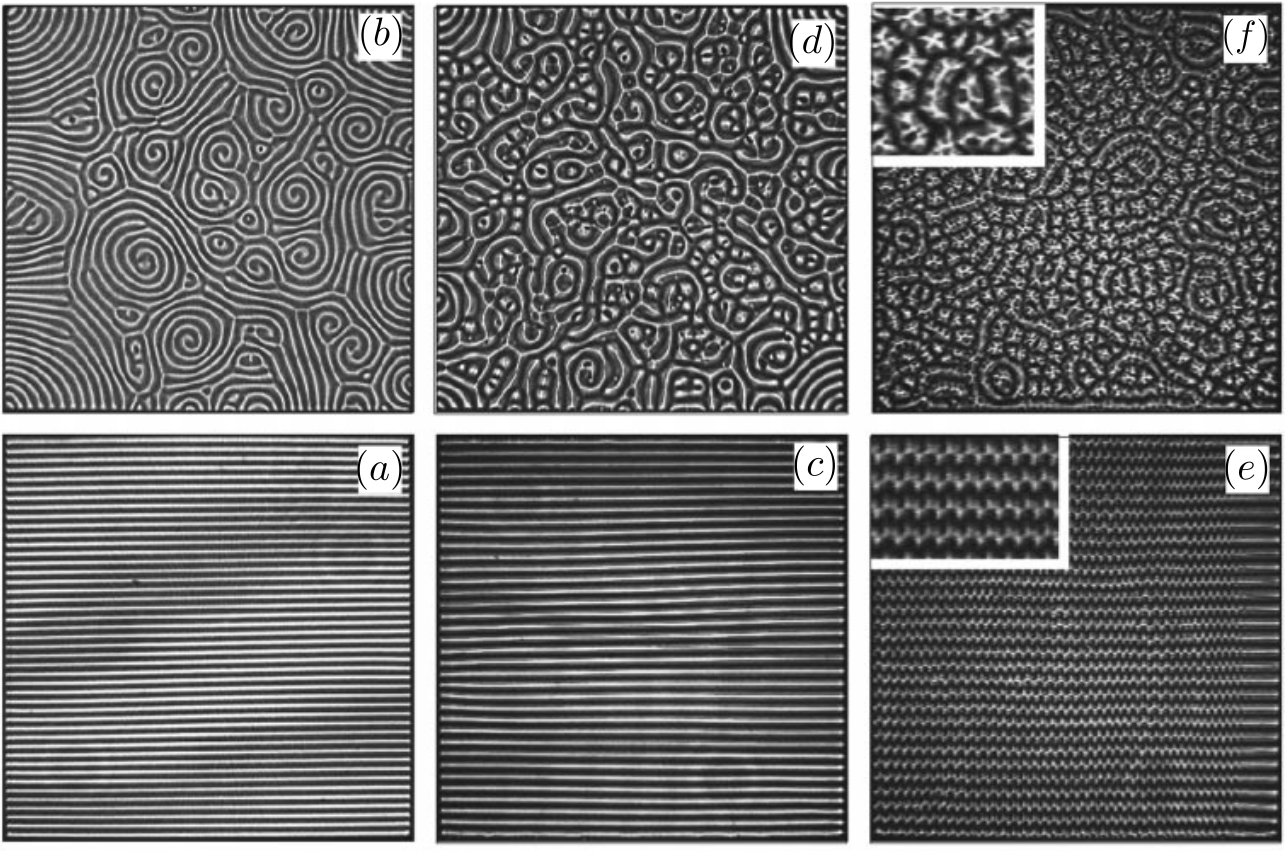
\includegraphics[width=\textwidth]{Background/Figures/bistability.png}
    \caption{The coexistence of spiral defect chaos (SDC, top row) and ideal straight rolls (ISRs, bottom row) at (a,b) $Ra = 3279$, (c,d) $Ra = 6832$ and (e,f) $Ra = 10384$. The domain size is $\Gamma = 50$ and $Pr = 1$, adapted from \cite{cakmur_bistability_1997}.}
    \label{fig:sdc_isr}
\end{figure}
However, the SDC attractor have been found to be unstable at $Pr = 4$, decaying towards ISRs over long periods \citep{bajaj_competition_1997}.
SDC has also been modalled in numerical simulations of the two-dimensional Swift-Hohenberg equations \citep{swift_hydrodynamic_1977,xi_spiral_1993,xi_spatiotemporal_1995,schmitz_spiral-defect_2002,karimi_exploring_2011}.
The critical Rayleigh number for the onset of SDC, $Ra_s$, depends on the domain's aspect ratio, and Prandtl number \citep{hu_convection_1995,bajaj_competition_1997,cakmur_transition_1997,bodenschatz_recent_2000}, and remain inconclusive.
% Investigations into quantifying the onset of SDC in terms of Rayleigh number remain inconclusive as it appears to depend on the domain's aspect ratio, and Prandtl number \citep{hu_convection_1995,bajaj_competition_1997,cakmur_transition_1997,bodenschatz_recent_2000}.
% The critical reduced Rayleigh number for the onset of SDC, $\varepsilon_s$, has been observed to decrease with increasing $\Gamma$, and increase with increasing $Pr$ \cite{hu1995a, hu1995b, bajaj1997, Cakmur97, bodenschatz2000}.
Notably, SDC has been reported in large domains ($\Gamma \gtrsim 20$), implying that there is a minimal $\Gamma$ for SDC to occur \citep{bodenschatz_recent_2000}, supporting the dependence of the $Ra_{s}$ on $\Gamma$.
The chaotic properties of SDC is also dependent of aspect ratio, where the leading Lyapunov exponents decreases with aspect ratio \citep{egolf_mechanisms_2000, paul_extensive_2007}.
Investigations into the spatial-temporal description of SDC such as the averaged roll-curvature \cite{hu_convection_1995}, probability distribution of spirals \cite{ecke_excitation_1995, liu_spiral-defect_1996} and correlation length-/time-scales \citep{morris_spiral_1993, morris_spatio-temporal_1996, cakmur_transition_1997} have been undertaken. 
Specifically, the correlation length-scales \citep{morris_spiral_1993, morris_spatio-temporal_1996, cakmur_transition_1997} scales exponentially with $Ra$, suggesting that onset of SDC from ISRs mimicks a phase transition.
Spatiotemporal chaotic behaviour similar to SDC has been found also in other pattern-formation systems such as rotational RBC \cite{hu_convection_1997}, dielectric barrier discharge \cite{dong_observation_2005} and advection diffusion reaction systems \cite{affan_spiral_2014}.

% Given the co-existence of ISRs and SDC in the parameter space of $\varepsilon$, it is known that they form bistability at $Pr \approx 1$ in a spatially extended domain, supported by experiments over a range of $\varepsilon(>0)$ \cite{Cakmur97}.
% The chaotic state of SDC is unstable at $Pr=4$, where multiple spiral patterns coarsen into a single spiral, before evolving into straight-curved rolls over a long period \cite{bajaj1997}.

% For large aspect ratios, $\Gamma \gtrsim  20$, convection rolls can exhibit spatiotemporal chaotic behaviour, known as spiral defect chaos (SDC) within the same $Ra$ range \citep{Morris93,Decker94,hu1995b,morris1996,Cakmur97,ahlers1998,egolf1998,chiam2003,vitral2020}.
% It is now established that both SDC and ISR can coexist at the same $Ra$, forming a bistable system confirmed experimentally \citep{Cakmur97}.

% HYSTERSIS
% Experimental investigations of RBC in moderate domain sizes ($\Gamma  = L/d \approx 14$ refers to the domain's aspect ratio) in rectangular (straight rolls) and cylinderical (concentric rolls) domains showed that the wavenumbers are confined within the Busse balloon.
% Depending on $Pr$, either mechanism could arise, increasing the effective roll wavenumber of the stability to adhere within the stability boundaries of the Busse balloon.
% For higher roll wavenumbers instabilities, the skewed-variose secondary instabilities arise, described by roll-pinching and merging where the effective roll-wavenumber is reduced to fall within the Busse balloon.
% At higher $Ra$, the oscillatory (OS) instability appears for $Pr \lesssim 1$ while the knotted stability appear for higher $Pr$.
% The oscillatory instability forms oscillatory ISRs reported by \cite{willis_oscillatory_1970}, while the knotted instability leads to spoke-liked covection patterns.
% , the cross roll (CR),  zig-zag and the well known Eckhaus secondary instabilties emerge.
% Lastly, the onset of a generic Eckhaus instability leads to either a roll destruction or emergence to stay within the Busse balloon.
% We will focus the secondary instabilities at $Pr = 1$ in this thesis.

% At $Pr \approx 1$, the secondary instabilities for large wavelengths are delimited by the cross-roll (CR) instability and the Eckhaus instability (not shown).
% The CR instability generates an addition roll orthogonal to the existing roll which increasing the effect roll wavenumber.
% Depending of the initial roll wavenumber, the Eckhaus instability either generates an additional or destroy rolls so that the stability boundaries are adhered to.
% The secondary instabilities for small wavelengths are delimited by the skewed-varicosed instability, where adjacent rolls pinches and merge wher a new ISR emerge adhering to the stability boundaries.

% For high Prandtl number fluids, the zig-zag instability occurs at small wavenumbers, causing wavy distortions.

 % long-wavelength modulation instabilities, where the disturbance wavenumber $|\mathbf{s}| \ll |\mathbf{q}|$ perturbs the ISR pattern. Depending on the direction and structure of the perturbation, one observes different instability types: the Eckhaus instability (ECK), involving modulations of roll spacing with $\mathbf{s} \parallel \mathbf{q}$; the zig-zag instability (ZZ), characterised by undulations along the roll axis with $\mathbf{s} \perp \mathbf{q}$; and the more general skewed varicose instability (SV), which encompasses both. For Prandtl numbers near unity ($Pr \approx 1$), SV instabilities delineate the high-wavenumber ($q$) boundary of the Busse balloon.

% In contrast, at low Prandtl numbers ($Pr \ll 1$), an oscillatory instability limits the stability region from above. This mode, marked by $\text{Im}(\omega(k)) \neq 0$ and $\mathbf{s} \approx \mathbf{q}$, leads to time-dependent behavior with propagating wave patterns and significant vertical vorticity. Additionally, short-wavelength instabilities can destabilize the ISR pattern through disturbances with $|\mathbf{s}| \approx |\mathbf{q}|$ but at a finite angle relative to $\mathbf{q}$. For $Pr \approx 1$, the cross-roll instability (CR) becomes prominent at small $q$, where new rolls form orthogonally to the original ones, preventing the development of overly short-wavelength patterns.

% Despite the idealised assumptions underlying the Busse balloon, experiments \citep[see][]{egolf_dynamical_1998} have demonstrated that its stability boundaries remain locally applicable to patches of ISR even in more disordered or weakly turbulent regimes. As such, the Busse balloon remains a central tool in understanding the transition from regular convection patterns to spatiotemporal complexity in Rayleigh–Bénard convection.
% Depending on the value of the Prandlt number, different types of secondary instabilities may arise, secondary instabilities may arise.
% % The secondary instabilities of thermal convection rolls are crucial for understanding the transition to more complex flow patterns.
% In low Prandtl number fluids, the oscillatory instability appears dominant, characterised by oscillations propagating along the ro, and the knot instability, a modification of the cross-roll instability that introduces a spoke pattern form of convectionlls.
% For intermediate $Pr$, skewed varicose instability, causing in a merging of neighbour rolls elongating the wavelength of the rolls.
% These instabilities, arising from different physical mechanisms related to momentum and heat transfer, dictate the stability and evolution of convection patterns as parameters like the Rayleigh and Prandtl numbers change.

% It is noted that weakly nonlinear stability analysis is only limited to $Ra$ slight above $Ra_c$ \citep{busse_oscillatory_1972}.
% As noted by \cite{busse_oscillatory_1972}, the applicability of weakly nonlinear analysis to slightly above onset, 
%which has been found to be a secondary instability of stationary convection rolls with complex eigenvalues.
% The theoretical foundations of performing stability analysis using expansion in powers of amplitude  (\emph{weakly nonlinear analysis}) was considered by \cite{eckhaus_studies_1965}, in which he applied it to the problem of parallel shear flows.
% The important contribution was that slightly above the onset, stable stationary rolls are found within the range of $Ra > Ra_c + 3\eta(\alpha - \alpha_c)^2$, where $\eta = \frac{1}{2}\frac{\partial Ra}{\partial \alpha}|_{Ra_c}$.
% \cite{busse_instabilities_1971} then extended the same technique to Rayleigh-B\'{e}nard convection, in which $\eta$ was found to depend on $Pr$.


% To complicate the subject further, ISRs appear to be an exception rather than the rule \citep{croquette_convective_1989-1} as multiple `non-ISR' states, in the form os squares, travelling/stationary targets, giant rotating spirals and oscillatory convection patterns have been found over the years \citep{croquette_convective_1989,croquette_convective_1989-1,plapp_dynamics_1998,hof_flow_1999,rudiger_pattern_2000,boronska_extreme_2010,boronska_extreme_2010-1}.
% For example, investigations of cylinderical RBC in small aspect-ratio revealed eight stationary statesand two oscillatory states.
% These findings were later supported by numerical experiments and bifurcation analyses.

% \begin{enumerate}
%     \item Saturated States
%     \item Busse balloon for Pr = 1
%     \item Skew-varicose, Eckhaus, Cross-roll instabilities
%     \item Low $Pr$ and high $Pr$.
%     \item What happens above the Busse balloon?
% \end{enumerate}
% 
% \begin{enumerate}
%     \item Statisitical description of spatial-temporal chaos (i.e correlation length, time etc..)
%     \item Challenge with quantifying the onset
% \end{enumerate}

% \subsection{Turbulent Rayleigh Benard: ultimate regime vs classical regime
% \begin{enumerate}
%     \item Onset of turbulence RBC
%     \item Introduce classical vs ultimate regime and scaling arguments of $Nu$.
% \end{enumerate}


%%%%%%%%%%%%%%%%%%%%%%%%%%%%%%%%%%
% Rayleigh Benard Poiseuille flows
%%%%%%%%%%%%%%%%%%%%%%%%%%%%%%%%%%

\section{Rayleigh-B\'{e}nard Poiseuille (RBP) flows}\label{sec:bkgrd_RBP}

% The RBP system consist of the primary instabilities of the RBC and RBP configurations and in the limiting cases, we observe the onset of convection rolls at $Ra_c = 1708$, and Tollmien Schlicting waves at $Re = 5772$.
\begin{figure}[h]
    \centering
    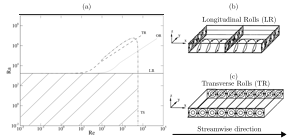
\includegraphics[width=\textwidth]{Background/Figures/RBP/RBP.pdf}
    \caption{(a) Neutral stability curves of longitudinal rolls (LR), oblique rolls (OR), transverse rolls (LR) and Tollmien-Schlicting (TS) waves, adapted from \cite{john_soundar_jerome_transient_2012}. The shaded area refers to damped perturbations. Sketch of (b) longitudinal and (c) transverse rolls, adapted from \cite{kelly_onset_1994}.}
    \label{fig:primary_instabilities}
\end{figure}

The neutral stability curves in the Rayleigh-B\'{e}nard Poiseuille (RBP) comprising of both plane Poisueuille flow (PPF) and Rayleigh-B\'{e}anrd convection (RBC) systems, are bounded by the onset of Tollmien-Schlicting waves at $Re_{c} = 5772.22$ \citep{orszag_accurate_1971}, and by the onset of convection rolls at $Ra_c = 1708$ \citep{pellew_maintained_1940}, respectively.
The imposed mean Poiseuille flow in the RBP system breaks the rotational invariance of the convection rolls, categorising them based on their orientation to the mean flow direction, namely: longitudinal ($\alpha= 0, \beta \neq 0$), transverse ($\alpha \neq 0, \beta = 0$) and oblique rolls ($\alpha \neq 0, \beta \neq 0$).
% Due to the imposed mean flow, the convection rolls are not rotationally invariant, and their orientation with respect to the mean matters.
% Generally, convection rolls that are aligned, diagonal and perpendicular to the mean flow are referred to longitudinal, oblique and transverse rolls.
The primary instabilities leading to these rolls were first investigated by \cite{gage_stability_1968} in an infinitely extended layer.
For the onset of longitudinal rolls, the linearised system reduces to that of RBC.
Hence, the critical Rayleigh number for the onset of longitudinal rolls remains the same, $Ra_{\parallel} = Ra_{c} = 1708.8$ with a critical wavenumber, $\alpha_{\parallel} = \alpha_{c} = 3.13$ \citep{pellew_maintained_1940, kelly_onset_1994}, independent of both Reynolds number, $Re$, and Prandtl number $Pr$.
In contrast, the onset of transverse rolls exhibits a critical Rayleigh number, $Ra_\perp = f(Re,Pr)$, that increases with $Re$ and is dependent on $Pr$ \citep{gage_stability_1968, muller_transversal_1992, nicolas_two-dimensional_1997}.
The critical Rayleigh number for the onset of obliqued rolls can be obtained by applying a Squire transformation \citep{squire_stability_1933} to the linearised problem for transverse rolls.
For a given $Ra$, the corresponding critical $Re$ for the onset of oblique rolls is higher than that of transverse rolls \citep{gage_stability_1968}.
% The critical Rayleigh number for the onset of obliqued rolls are obtained by performing a Squire transformation on the linearised transverse roll system where for a given $Ra$, the critical $Re$ of oblique rolls is higher than the critical $Re$ for transverse rolls \citep{gage_stability_1968}.
The neutral stability curves associated with the transverse rolls (TR), oblique rolls (OR) and longitudinal rolls (LR) are shown in figure \ref{fig:primary_instabilities}.

Experimental observations of the onset of longitudinal rolls have been reported in channels with large transverse aspect ratios (i.e span-to-depth) \citep{akiyama_experiments_1971,ostrach_heat_1975,fukui_longitudinal_1983}, while the onset of transverse rolls are observed in narrower channels \citep{luijkx_existence_1981,ouazzani_etude_1989,ouazzani_etude_1990}.
Indeed, linear stability analysis conducted for finite channels revealed that critical Rayleigh number $Ra_\parallel$ remains independent for transverse aspect ratios greater than five, and increases quickly below that.
Therefore, the critical Rayleigh number for onset of transverse rolls, $Ra_\perp$, is lower than $Ra_\parallel$ in narrow channels for small Reynolds numbers \citep{nicolas_linear_2000}, providing support for the preference of transverse rolls in narrow channels.
% Indeed, linear stability analysis of narrow channel reveal that the $Ra_{\parallel}$ are increased relative to the $Ra_\perp$ for small $Re$ \citep{nicolas_linear_2000}.
\cite{ouazzani_etude_1990} reported laminar Poiseuille flow in the $Ra, Re$ parameter space where transverse rolls are expected based on temporal linear stability analysis.
% However, linear temporal stability analysis failed to explain the experimental results from \cite{ouazzani_etude_1990}, where a laminar Poiseuille is observed in the parameter space where transverse rolls are expected.
This contraction was address by \cite{muller_transversal_1992}, who showed that transverse rolls can be either convectively or absolutely unstable, and the boundary between them matches with the experimental results of \cite{ouazzani_etude_1990}.
By considering the response from three-dimensional impulse, \cite{carriere_convective_1999} further demostrated that the longitudinal rolls, unlike the transverse rolls, are always convectively unstable.
% The critical Rayleigh number for oblique and transverse rolls matches that of RBC at $Re=0$ due to horizontal isotropy, but increases as $Re$ increases, depending on $Pr$, i.e., $Ra_{\perp} = f(Re,Pr)
Nonmodal stability analysis of subcritical RBP, $Ra < Ra_c, Re < Re_{c}$, performed by \cite{john_soundar_jerome_transient_2012} revealed that the optimal transient growth is primarily dominanted by streamwise rollers of plane Poiseuille flow \citep{reddy_energy_1993}, with a spanwise wavenumber of $\beta_{opt} \approx 2.05$.
The maximum amplifcation factor, $G_{max}$ increases modestly with $Ra$, and the critical wavenumber approaches, $\alpha_{\parallel}$, indicative of longitudinal rolls.
% Nonmodal stability analyses of subcritical RBP indicate that the optimal transient growth $G_{max}$ increases gradually with $Ra$.
% The wavenumber of the optimal initial conditions, $\beta_{max}$, resembles that observed in shear flows \citep{reddy_energy_1993}, and gradually approaches the critical wavenumber of convection rolls, $\alpha_{\parallel}$, as $Ra$ increases \citep{john_soundar_jerome_transient_2012}.
% For $Re > 0$, the longitudinal rolls appear as the dominant primary instability \citep{gage_stability_1968}.
Since longitudinal rolls are the dominant primary instability for $Re > 0$ in infinite domains, their secondary stability have been analysed by \cite{clever_instabilities_1991}.
Their study revealed the presence of a secondary, time-dependent wavy instability near $Re \sim 100$ \citep{clever_instabilities_1991}, leading to the onset of tertiary solutions in the form of wavy rolls.
These have been observed experimentally and was found to be convectively unstable \citep{pabiou_observations_2003, pabiou_wavy_2005, nicolas_characterisation_2010}.
\cite{clever_instabilities_1991} also speculated that the wavy rolls are less efficient at transporting heating than longitudinal rolls at the same control parameters, confirmed numerically \citep{nicolas_influence_2012}.
The impact of finite transverse aspect ratios on the onset of wavy rolls have been also studied \citep{xin_stability_2006, nicolas_characterisation_2010}, where the critical $Ra$ was found to be approximatgely 1.5 times higher than that in an infinite domain \cite{clever_instabilities_1991}.
The influence of external excitations on the development length of wavy rolls have been explored.
An increase in external excitation amplitude have shown to reduced the required development length of wavy rolls \citep{nicolas_characterisation_2010,nicolas_influence_2012}.
More recently, studies of turbulent RBP flows showed that shear-driven turbulence can enhance heat fluxes \citep{scagliarini_heat_2014, scagliarini_law_2015, pirozzoli_mixed_2017}.
% In finite streamwise extensions of RBP flows, the onset of convection rolls and the heat flux variations due to entrance effects have been investigated \citep{mahaney_effect_1988,lee_effect_1991,nonino_laminar_1991}.
Extensions of the RBP configuration, such as flows over wavy walls or with sinusoidal thermal forcing have been investigated, potentially offering a reduction in drag and enhancing heat transport \citep{hossain_drag_2012,hossain_drag_2016,hossain_role_2020}.
% RBP flows with sinusoidal heating and wavy walls have also been studied \citep{hossain_spectral_2021}.
For a comprehensive overview of RBP flows, the reader is referred to the reviews by \cite{kelly_onset_1994} and \cite{nicolas_revue_2002}.

%%%%%%%%%%%%%%%%
% THESIS OUTLINE
%%%%%%%%%%%%%%%%

\subsection{Thesis Outline}\label{sec:thesis_outline}

% The governing equations of the fluid motion in given by the Navier-Stokes equations with Boussinessq approximations,
% \begin{equation}
%     \frac{\partial \mathbf{u}}{\partial t} + (\mathbf{u} \cdot \nabla) \mathbf{u} = -\frac{1}{\rho} \nabla p + \nu \nabla^2 \mathbf{u} + g\beta(T-T_0).
% \end{equation}`
% \begin{equation}
%     \frac{\partial T}{\partial t} + (\mathbf{u} \cdot \nabla)T = \kappa \nabla^2 T,
% \end{equation}
% \begin{equation}
%     \nabla  \cdot \mathbf{u} = 0.
% \end{equation}
% with arbitrary Dirichlet and Neumann boundary conditions.
% \begin{equation}
%     \mathbf{u}_d, p_d, T_d \in \Omega_d, \quad \nabla\mathbf{u}_N, p_N, T_N \in \partial\Omega_N.
% \end{equation}
% where $\mathbf{u}, T, p$ refers to the velocity, temperature and pressure fields, primitive variables that are not known a priori and $\rho, \nu, \kappa$ refers to the properties of the fluid, namely, density, kinematic viscosity and thermal diffusivity.
% For a given set of fluid properties $\rho, \nu, \kappa$ and geometric properties $L^*, t^*, u^*$ referring to an arbitrary length-, time- and velocity-scale, we are primarily interested in the behaviour of the fluid i.e if its laminar or turbulent.
% In other words, we have a six control parameters that describes a fluid flow of interest.
% To reduce the number of control parameters, we can suitably nondimensionalise the primitive variables by a velocity scale $u_c$, length scale, $L_x$, and time scale $u_c/L_x$, where $u_c$ refers to the centreline velocity of a laminar flow and $L_x$ refers to the streamwise length of the domain.
% The nondimensional equations with Boussienessq approximations are now given as,
% \begin{equation}
%     \frac{\partial \mathbf{u}}{\partial t} + (\mathbf{u}\cdot\nabla)\mathbf{u} = -\nabla p + \frac{1}{Re}\nabla^2 \mathbf{u} + \frac{Ra}{Re^2Pr} \theta
% \end{equation}
% \begin{equation}
%     \frac{\partial \theta}{\partial t} + (\mathbf{u} \cdot \nabla)\theta = \frac{1}{RePr}\nabla^2 \theta,
% \end{equation}
% \begin{equation}
%     \nabla \cdot \mathbf{u} = 0.
% \end{equation}
% where $\mathbf{u}, \theta, p$ refers to the nondimensionalised velocity, temperature and presure.
In this thesis, I am particularly focused on the transition behaviour of fluid flow driven by shear and bouyancy, addressing questions related to the onset of instabilities due to shear and buoyancy, and the (possible) competitive between shear and buoyancy driven instabilities.
I would like to preface that while this thesis is dealing with onset of instabilities, it does not clearly indicate that the onset of such instabilities necessarily lead to turbulence, hence, for terminology sake, we shall be looking into transitional regimes where the fluid neither laminar nor turbulent.
The main motivations are two-folds, both from an academic and applied point-of-view. 
Within academia, the onset and transition to turbulence in Rayleigh-B\'{e}nard Poiseuille flows remains poorly understand.
Whilst there had been significant progress in our understand of transition to turbulence in independent setups, Rayleigh-B\'{e}nard convection and plane Poiseuille flows, their combined effects are not known.
The thesis is structured into the follow, Chapter 1 is the introduction with literature review, chapter 2 methodology assosicated with the spectral/\emph{hp}-element method, chapter 3 with results related to the the Rayleigh and Reynolds number sweep, chapter 4 with a specific focus on the bistability between spiral defect chaos and ideal straight rolls and finally chapter 5 with concluding remarks.

\begin{enumerate}
   \item Academic motivation - flow structures, statistics, transition.
   \item Application motivation - shear, heat transfer. Chip cooling, thin-film fabrication and atmospheric boundary layer.
\end{enumerate}
We seek to investigate the influence of unstable stratification quantified by Rayleigh number $Ra$, on the behaviour tuburlent-laminar bands. 
The onset of convection occurs at a critical Rayleigh number of $Ra_c > 1708$, in the form of a pair of convection rolls.
When aligned in the streamwise direction, the convection rolls are seemingly analogous to a pair of counter-rotating vortices, an optimal initial condition for transient growth. 
Our investigation naturally answers a few questions related to turbulent-laminar bands.
For example, does the onset of turbulent-laminar bands, $Re_{cr}$ decrease with increasing $Ra$?
Do $Ra$-effects influence the structure of turbulent-laminar bands i.e band angle/width? 

The answers to our research will have important implications Rayleigh-B\'{e}nard Poiseuille flows, ubiquitous in atmospheric, geophysical and engineering flows.
